\problemname{\problemyamlname}

%\illustration{0.3}{image.jpg}{Caption of the illustration (optional). CC BY-NC 2.0 by X on Y}
% Source: URL to image.

% optionally define variables/limits for this problem

Jérôme et ses deux coéquipiers doivent se rendre aux KARWa à l'UMONS.
Malheureusement, ils se sont trompés d'université et ont atterri à l'UCLouvain !
Ils sont pressés par le temps et demandent à leur ami Nicolas expert des cartes et des plus courts chemins qui a sa disposition une carte avec $n$ gares et $m$ lignes de trains bidirectionnelles (qui vas dans les deux sens), prenant chacun un temps $w$.
Pouvez-vous déterminer s'ils auront le temps d'arriver à l'heure ?

L'UCLouvain est représentée par l'intersection $1$ et l'UMONS par l'intersection $n$.
Un chemin est garanti entre les deux universités.
\begin{figure}[h]
	\centering
	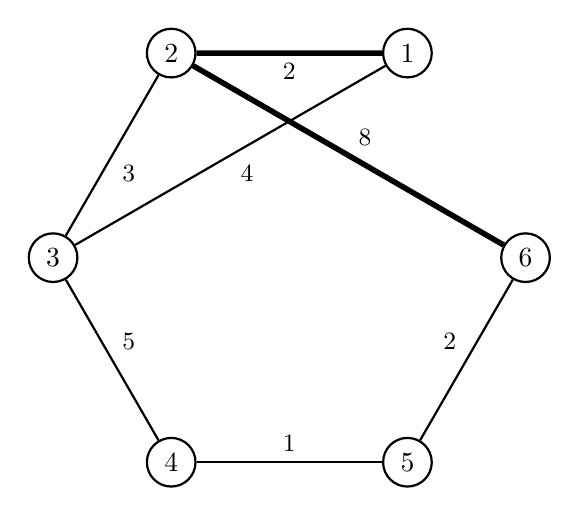
\begin{tikzpicture}[auto,node distance=2cm,thick]
		\tikzset{edge/.style = {draw, -}}
		\tikzset{weight/.style = {font=\small}}
		
		% nodes
		\foreach \i in {1,...,6}
			\node[circle,draw] (\i) at (360/6*\i:3) {\i};
		
		% edges and weights
		\draw[edge] (1) -- node[weight]{2} (2);
		\draw[edge] (1) -- node[weight]{4} (3);
		\draw[edge] (2) -- node[weight]{3} (3);
		\draw[edge] (2) -- node[weight]{8} (6);
		\draw[edge] (3) -- node[weight]{5} (4);
		\draw[edge] (4) -- node[weight]{1} (5);
		\draw[edge] (5) -- node[weight]{2} (6);
		
		% path from 1 to 6 in bold
		\draw[line width=2pt] (1) -- (2) -- (6);
		
		% uncomment the following line to add labels to the nodes
		% \foreach \i in {1,...,6} \node at (360/6*\i:3.5) {\i};
		\end{tikzpicture}
		
\caption[short]{Exemple 1 : avec le chemin de 1 à 6 en gras}
\end{figure}
	

\begin{Input}
	L'entrée consiste en :
	\begin{itemize}
		\item une ligne de deux entiers $n$ et $m$ ($2 \le n, m \le 10^6$), où $n$ est le nombre d'intersections et $m$ le nombre de liaisons,
		\item $m$ lignes contenant chacune 3 entiers $u$ ($1 \le u \le n$), $v$ ($1 \le v \le n$), et $w$ ($1 \le w \le 10^6$), représentant une liaison bidirectionnelle entre $u$ et $v$, avec un poids $w$.
	\end{itemize}
\end{Input}

\begin{Output}
	Une ligne contenant la longueur du plus court chemin entre $1$ et $n$.
\end{Output}
